\documentclass{beamer}
%Information to be included in the title page:
% \title{Sample title}
% \author{Anonymous}
% \institute{Overleaf}
\usepackage{xcolor}
\usepackage{booktabs}
\usepackage{graphicx}
\usepackage{subcaption}
\usepackage[]{hyperref}

\usetheme[]{default}
\begin{document}
\renewcommand{\d}{\: \mathrm{d} }
\newcommand{\e}{\mathrm{e}}


\title[] {Recitation Class 5}

\author[lzx]{Zexi Li}

\institute[email]{lzx12138@sjtu.edu.cn}

\date{2021.06.22}

\frame{\titlepage}

\AtBeginSection[]
{
    \begin{frame}
        \frametitle{Table of Contents}
        \tableofcontents[currentsection]
    \end{frame}
}

\begin{frame}
    \frametitle{Outline}
    \tableofcontents
\end{frame}

\section{Chapter 6 Nonequilibrium Excess Carriers in Semiconductors}
    \begin{frame} \frametitle{Notations in Chapter 6}
        \begin{figure}[H]
            \centering
            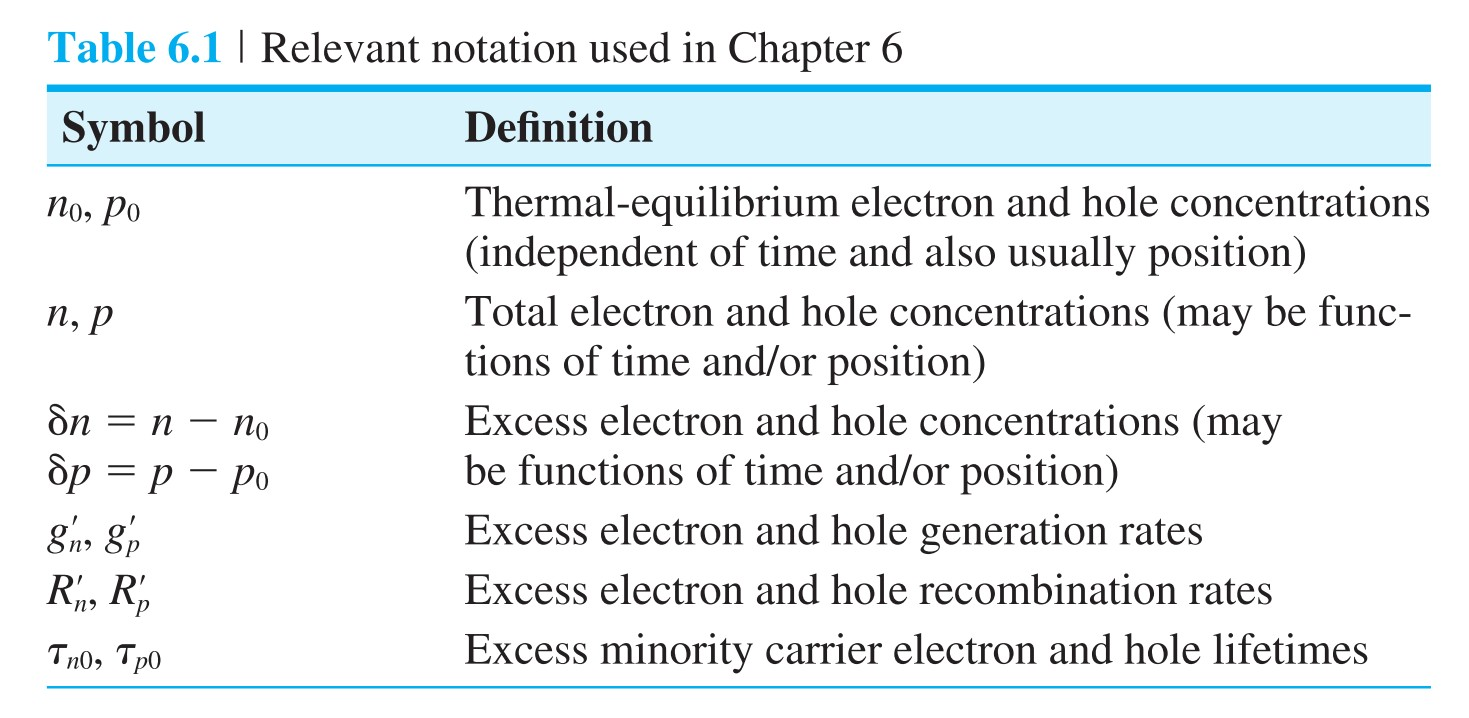
\includegraphics[width=0.9\linewidth]{Notations.jpg}
            \label{fig:Notations.jpg}
        \end{figure}
    \end{frame}
    \begin{frame} \frametitle{Electron-hole Generation \& Recombination}
        \begin{figure}[H]
            \centering
            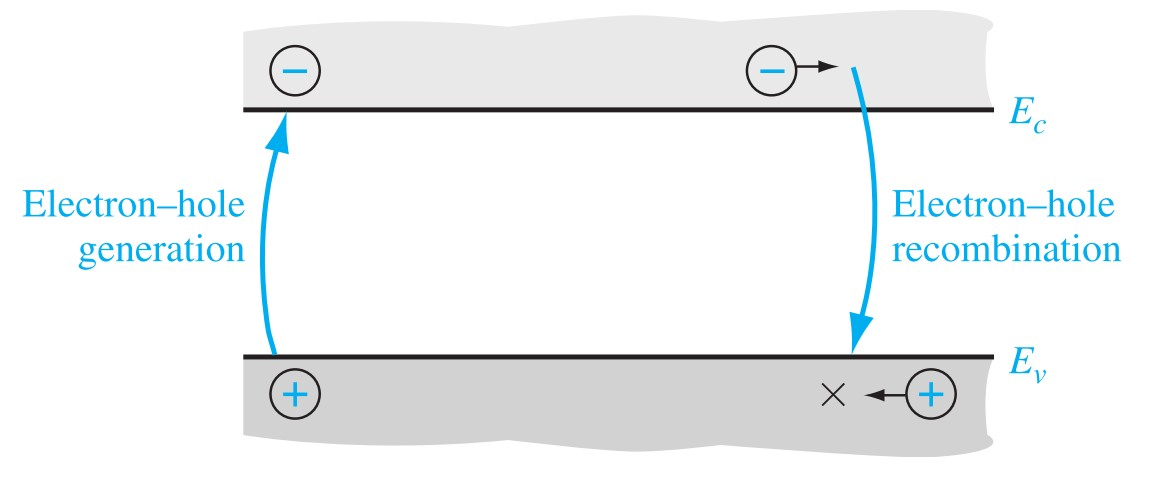
\includegraphics[width=0.6\linewidth]{Generation-recombination.jpg}
            \label{fig:Generation-recombination.jpg}
        \end{figure}
        \begin{equation*}
            G_{n0} = G_{p0}, \quad R_{n0} = R_{p0}
        \end{equation*}
    \end{frame}

    \begin{frame} \frametitle{Thermal-equilibrium}
        \textcolor{blue}{Thermal-equilibrium}: the net carrier concentrations are independent of time, which means that the generation and recombination of electrons and holes are equal.
        \begin{equation*}
            G_{n0} = G_{p0} = R_{n0} = R_{p0}
        \end{equation*}

        \textcolor{blue}{Nonequilibrium}: 
        
        \begin{minipage}{\linewidth}
            \begin{minipage}{0.5\linewidth}
                \begin{equation*}
                    \begin{aligned}
                        n &= n_0 + \delta n \\
                        p &= p_0 + \delta p
                    \end{aligned}
                \end{equation*}
                \par Note that $np \neq n_0 p_0 = n_i^2$.
            \end{minipage}
            \begin{minipage}{0.49\linewidth}
                \begin{figure}[H]
                    \centering
                    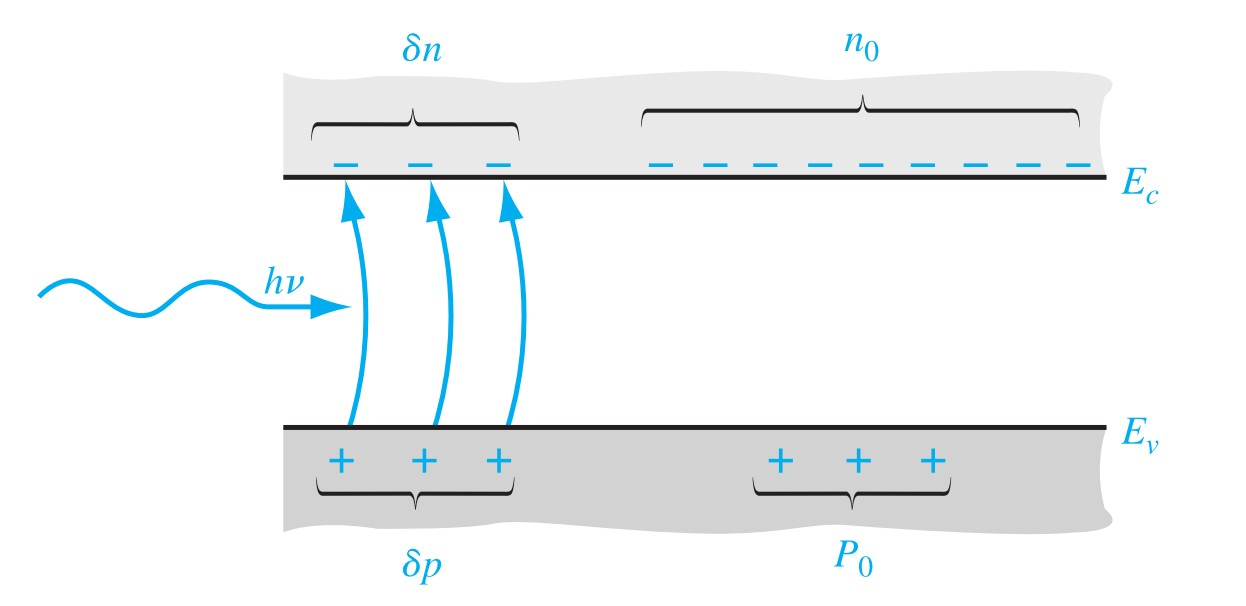
\includegraphics[width=\linewidth]{Photons-generation.jpg}
                    \caption{Creation of excess electron and hole densities by photons}
                    \label{fig:Photons-generation.jpg}
                \end{figure}
            \end{minipage}
        \end{minipage}
    \end{frame}
    \begin{frame} \frametitle{Net Recombination Rate}
        % TODO: derivation
        n-type:
        \begin{equation*}
            R^\prime_n = R^\prime_p = \frac{\delta p(t)}{\tau_{p0}}
        \end{equation*}
        p-type:
        \begin{equation*}
            R^\prime_n = R^\prime_p = \frac{\delta n(t)}{\tau_{n0}} 
        \end{equation*}
    \end{frame}

    \begin{frame} \frametitle{Quasi-Fermi Energy Level}
        \begin{equation*}
            \begin{aligned}
                n_0 + \delta n &= n_i \exp \left( \frac{E_{Fn} - E_{Fi}}{kT}  \right) \\
                p_0 + \delta p &= n_i \exp \left( \frac{E_{Fi} - E_{Fp}}{kT}  \right) \\
            \end{aligned}
        \end{equation*}
        \begin{figure}[H]
            \centering
            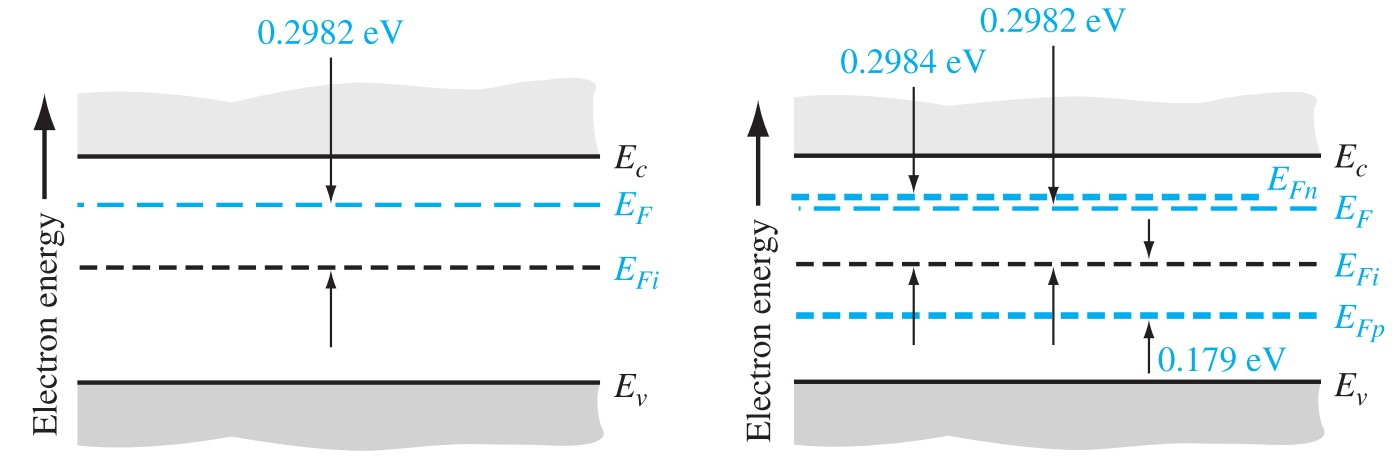
\includegraphics[width=\linewidth]{Quasi-fermi-level.jpg}
            \label{fig:Quasi-fermi-level.jpg}
        \end{figure}
    \end{frame}

    \begin{frame} \frametitle{Question}
        \textcolor{blue}{Why we only consider minority excess carrier?} \\
        \par Consider the case where we have a n-type silicon semiconductor, with $n_0 = 10^{17}cm ^{-3}$, and $p_0 = n_i^2 / n_0 = 2250cm^{-3}$. And the excess carrier $\delta n = 10^{14} cm^{-3}$, which is only $0.1\%$ of $n_0$. However, $\delta p = \delta n = 10^{14} cm^{-3}$, which is greatly larger than $p_0$.
        \par You can also have such feeling from the Quasi-Fermi Energy Level diagram that $E_{Fn}$ is close to $E_F$ while $E_{Fp}$ changes a lot.
    \end{frame}

    \begin{frame} \frametitle{Excess Carrier Lifetime}
        \begin{equation*}
            \boxed{R_n = R_p = \frac{C_n C_p N_t (np - n_i^2)}{C_n (n + n^\prime) + C_p(p + p^\prime)} \equiv R}
        \end{equation*}
        where $n^\prime = N_c \exp\left[ - \dfrac{E_c - E_t}{kT}  \right],   \qquad p^\prime = N_v \exp \left[ - \dfrac{E_t - E_v}{kT}  \right]$
    \end{frame}

    \begin{frame} \frametitle{Surface Effects}
        % TODO
        \begin{figure}[H]
            \centering
            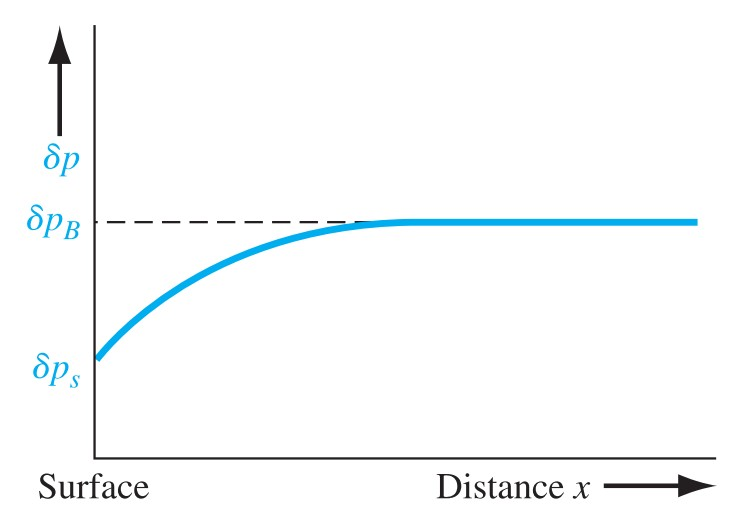
\includegraphics[width=0.6\linewidth]{Suerface-concentration.jpg}
            \label{fig:Suerface-concentration.jpg}
        \end{figure}
        
        \begin{equation*}
            \begin{aligned}
                \boxed{- D_p \left. \left[ \hat{n} \cdot \frac{\d (\delta p)}{\d x}  \right] \right|_{\text{surf}} = s \; \delta p |_{\text{surf}}}
            \end{aligned}
        \end{equation*}
    \end{frame}

    \begin{frame} \frametitle{Time-dependent Continuity Equation}
        \begin{equation*}
            \boxed{
                \begin{aligned}
                    D_n \frac{\d^2 n}{\d x^2} + \mu_n \left( E \frac{\d n}{\d x} + n \frac{\d E}{\d x}  \right) + g_n - \frac{n}{\tau_{nt}} = \frac{\d n}{\d t} \\
                    D_p \frac{\d^2 p}{\d x^2} - \mu_p \left( E \frac{\d p}{\d x} + p \frac{\d E}{\d x}  \right) + g_p - \frac{p}{\tau_{pt}} = \frac{\d p}{\d t} \\
                \end{aligned}
            }
        \end{equation*}
        \par For homogeneous semiconductor, $n(x) = n_0 + \delta n(x)$, the equation can be simplified to 
        \begin{equation*}
            \boxed{
                \begin{aligned}
                    D_n \frac{\d^2 (\delta n)}{\d x^2} + \mu_n \left( E \frac{\d (\delta n)}{\d x} + n \frac{\d E}{\d x}  \right) + g_n - \frac{n}{\tau_{nt}} = \frac{\d (\delta n)}{\d t} \\
                    D_p \frac{\d^2 (\delta p)}{\d x^2} - \mu_p \left( E \frac{\d (\delta p)}{\d x} + p \frac{\d E}{\d x}  \right) + g_p - \frac{p}{\tau_{pt}} = \frac{\d (\delta p)}{\d t} \\
                \end{aligned}
            }
        \end{equation*}
    \end{frame}

    \begin{frame} \frametitle{Equation Simplification}
        \begin{figure}[H]
            \centering
            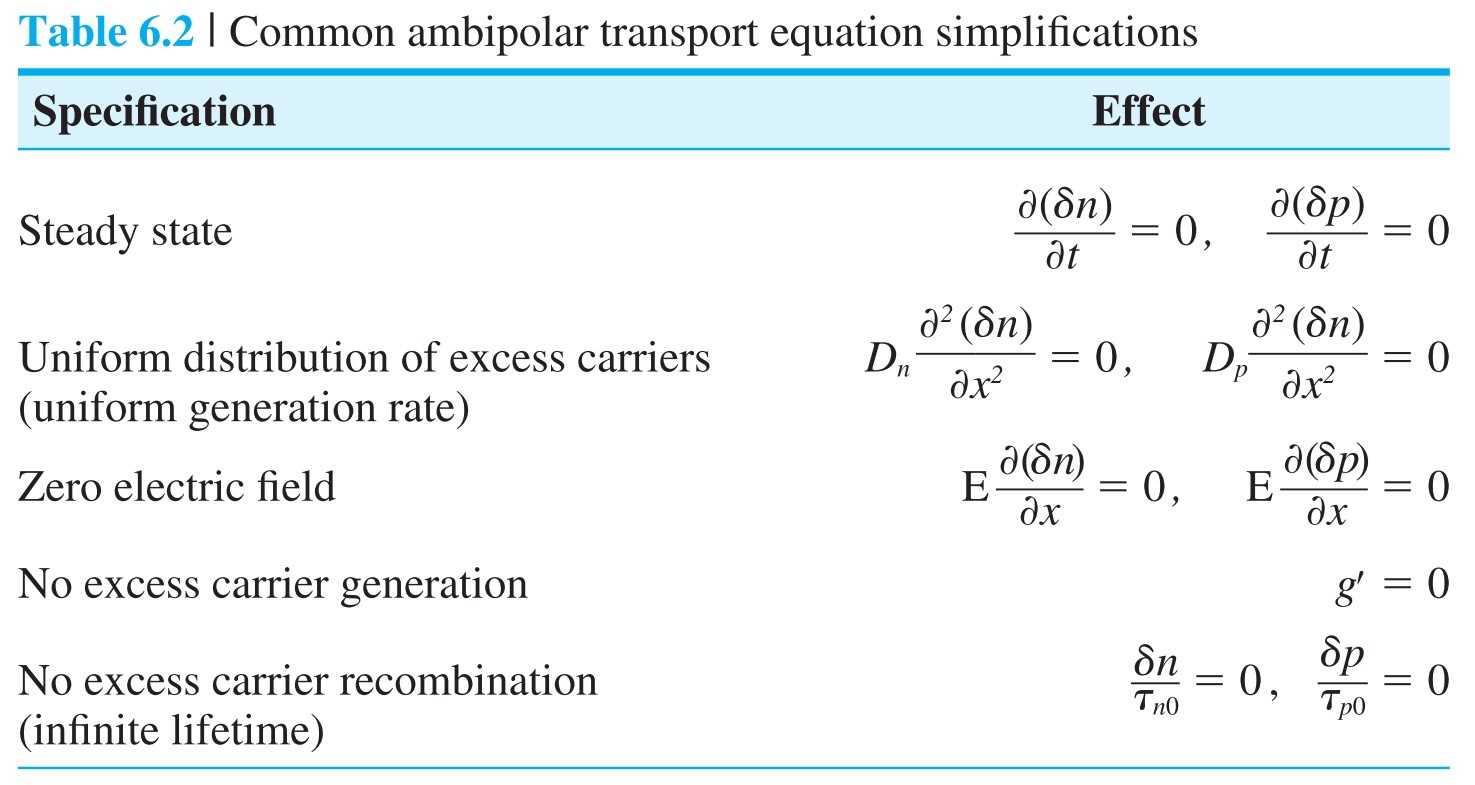
\includegraphics[width=0.9\linewidth]{Equation-simplification.jpg}
            \label{fig:Equation-simplification.jpg}
        \end{figure}
    \end{frame}


    % TODO: check equations in these three examples
    \begin{frame} \frametitle{Example I}
        \par Given a piece of p-type uniformly doped semiconductor in contact with two metal electrodes separated by a length of $L$, forming a photoconductor device. The light illumination will create electron-hole pairs at a generation rate of $g$. The minority carrier recombination lifetime is $\tau_0$. Find the analytical distribution of the excess minority electrons at zero external bias. Note that light illumination will not create excess carriers in metals. \\[3em]
        \begin{minipage}{\linewidth}
            \begin{minipage}{0.3\linewidth}
                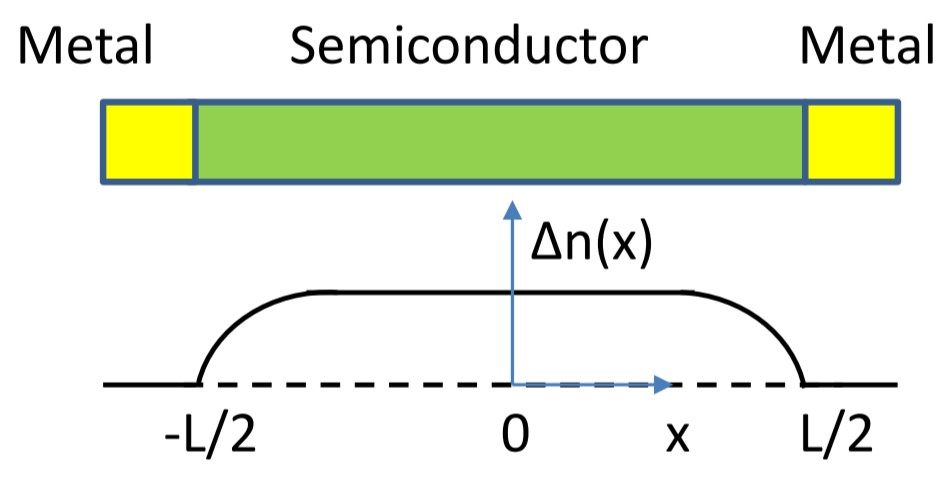
\includegraphics[width=\linewidth]{Example-1.jpg}
            \end{minipage}
            \begin{minipage}{0.69\linewidth}
                \resizebox*{\textwidth}{!}{ %
                    $ D_n \dfrac{\d^2 (\delta n)}{\d x^2} + \mu_n \left( E \dfrac{\d (\delta n)}{\d x} + n \dfrac{\d E}{\d x}  \right) + g_n - \dfrac{n}{\tau_{nt}} = \dfrac{\d (\delta n)}{\d t} $
                }
            \end{minipage}
        \end{minipage}
    \end{frame}

    \begin{frame} \frametitle{Example II}
        \par A light beam is illuminated on the surface of a silicon wafer, generating excess carriers $\Delta p_0$ at the surface ($x = 0$). The wafer is placed in a constant electric field with a known intensity $E$. We assume there is no external generation inside the wafer. The thickness of the wafer is infinite. Find the excess minority carriers at equilibrium as a function of the distance away from the surface ($x = 0$). Small injection condition is always maintained and the wafer is uniformly doped as $N_d$. \\[3em]
        \begin{minipage}{\linewidth}
            \begin{minipage}{0.3\linewidth}
                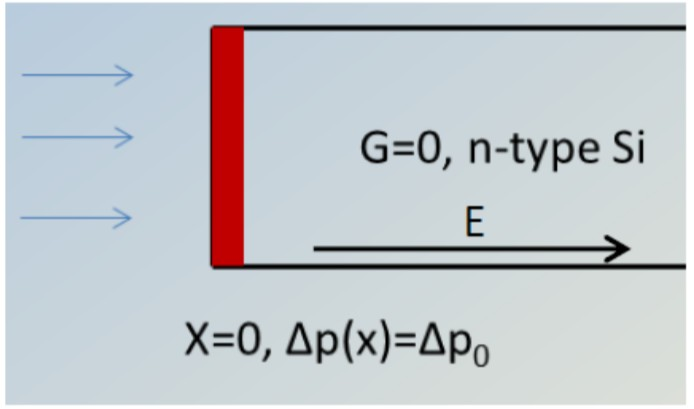
\includegraphics[width=\linewidth]{Example-2.jpg}
            \end{minipage}
            \begin{minipage}{0.69\linewidth}
                \resizebox*{\textwidth}{!}{ %
                    $ D_p \dfrac{\d^2 (\delta p)}{\d x^2} - \mu_p \left( E \dfrac{\d (\delta p)}{\d x} + p \dfrac{\d E}{\d x}  \right) + g_p - \dfrac{p}{\tau_{pt}} = \dfrac{\d (\delta p)}{\d t} $
                }
            \end{minipage}
        \end{minipage}
    \end{frame}
    % \begin{frame} \frametitle{Example II}
    %     \par Consider a bar of p-type silicon that is uniformly doped to a value of $N_a = 2 \times 10^{16} cm^{-3}$ at $T = 300 K$. The applied electric field is zero. A light source is incident on the end of the semiconductor as shown in figure. The steady-state concentration of excess carriers generated at $x = 0$ is $\delta p(0) = \delta n(0) = 2 \times 10^{14} cm^{-3}$. Assume the following parameters: $\mu_n = 1200 cm^{2} /V-s$, $\mu_p = 400 cm^2 / V-s$, $\tau_{p0}$
    % \end{frame}

    \begin{frame} \frametitle{Example III}
        \par Consider a p-type semiconductor that is homogeneous and infinite in extent. Assume a zero applied electric field. For a one-dimensional crystal, assume that excess carriers are being generated at $x = 0$ only, as indicated in Figure below. The excess carriers being generated at $x = 0$ will begin diffusing in both the $+x$ and $-x$ directions. Calculate the steady-state excess carrier concentration as a function of $x$. \\[2em]
        \begin{minipage}{\linewidth}
            \begin{minipage}{0.3\linewidth}
                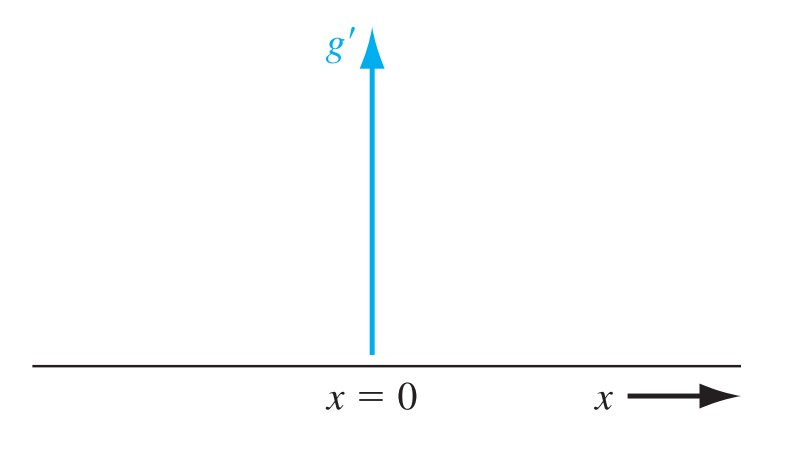
\includegraphics[width=\linewidth]{Example-3.jpg}
            \end{minipage}
            \begin{minipage}{0.69\linewidth}
                \resizebox*{\textwidth}{!}{ %
                    $ D_n \dfrac{\d^2 (\delta n)}{\d x^2} + \mu_n \left( E \dfrac{\d (\delta n)}{\d x} + n \dfrac{\d E}{\d x}  \right) + g_n - \dfrac{n}{\tau_{nt}} = \dfrac{\d (\delta n)}{\d t} $
                }
            \end{minipage}
        \end{minipage}
    \end{frame}

    \begin{frame} \frametitle{General Solutions -- t}
        \begin{itemize}
            \item 
                \begin{equation*}
                    \frac{\d (\delta p)}{\d t}  = - \frac{\delta p}{\tau_{p0}} 
                \end{equation*}
                solution:
                \begin{equation*}
                    \color{magenta} \delta p(t) = \delta p(0) \e^{- t/ \tau_{p0}} 
                \end{equation*}
            \item 
                \begin{equation*}
                    g^\prime - \frac{\delta p}{\tau_{p0}} = \frac{\d (\delta p)}{\d t}  
                \end{equation*}
                solution:
                \begin{equation*}
                    \color{magenta} \delta p(t) = g^\prime \tau_{p0} \left( 1 - \e^{- t / \tau_{p0}}  \right)
                \end{equation*}
        \end{itemize}
    \end{frame}

    \begin{frame} \frametitle{General Solutoins -- x}
        \begin{itemize}
            \item \begin{equation*}
                    D_n \frac{\d ^2 (\delta n)}{\d x^2} - \frac{\delta n}{\tau_{n0}} = 0
                \end{equation*}
                solution:
                \begin{equation*}
                    \color{magenta}
                    \delta n(x) = A \e^{- x/L_n} + B \e^{x/L_n}, \quad L_n = \sqrt{D_n \tau_{n0}}
                \end{equation*}
                special:
                \begin{equation*}
                    \color{magenta}
                    \delta n(x) = 
                    \left\{
                        \begin{aligned}
                            \delta n(0) \e^{-x / L_n}, &x \ge 0 \\
                            \delta n(0) \e^{+x/L_n}, &x \le 0
                        \end{aligned}
                    \right.
                \end{equation*}

            \item \begin{equation*}
                    D_p \frac{\d ^2 \delta p}{\d x^2} - \frac{\delta p}{\tau} + G_{ex} = 0
                \end{equation*}
                solution:
                \begin{equation*}
                    \color{magenta}
                    \delta p(x) = A \exp(\lambda x) + g \tau, \quad \lambda = \pm \frac{1}{\sqrt{D_p \tau}} 
                \end{equation*}
        \end{itemize}
    \end{frame}

    \begin{frame} \frametitle{General Solutions -- E}
        \begin{itemize}
            \item \begin{equation*}
                    D_p \frac{\d^2 (\delta p)}{\d x^2} - \mu_p E_0 \frac{\d (\delta p)}{\d x} - \frac{\delta p}{\tau_{p0}} = \frac{\d (\delta p)}{\d t}  
                \end{equation*}
                solution:
                \begin{equation*}
                    \color{magenta}
                    \delta p(x, t) = \frac{\e^{-t/\tau_{p0}} }{\left( 4 \pi D_p t \right)^{1/2}} \exp\left[ \frac{-\left(x - \mu_p E_0 t\right)^2}{4 D_p t}  \right]
                \end{equation*}
        \end{itemize}
    \end{frame}

    \begin{frame} \frametitle{General Soluitons -- E}
        \begin{itemize}
            \item \begin{equation*}
                    D_p \frac{\d^2 \delta p}{\d x^2} - \mu_p E \frac{\d \delta p}{\d x} - \frac{\delta p}{\tau} = 0 
                \end{equation*}
                solution:
                \begin{equation*}
                    \color{magenta}
                    \begin{aligned}
                        & \delta p(x) = A \exp\left( \lambda x \right) + C \\
                        & \lambda = \frac{L_p(E) \pm \sqrt{L_p^2 (E) + 4 L_p^2}}{2 L_p^2},\quad L_p = \sqrt{\tau D_p},\quad L_p(E) = \tau \mu_p E
                    \end{aligned}
                \end{equation*}
                special:
                \begin{minipage}{\linewidth}
                    \resizebox*{\textwidth}{!}{ %
                        $
                        \color{magenta}
                        \delta p(x) = \delta p(0) \exp \left[ \dfrac{L_p(E) \pm \sqrt{L_p^2 (E) + 4 L_p^2}}{2 L_p^2} x \right] = \left\{
                            \begin{aligned}
                                &\delta p(0) \exp \left( - \dfrac{x}{L_p}  \right), &\text{ if } L_p(E) \ll L_p \\
                                &\delta p(0) \exp \left( - \dfrac{x}{L_p(E)}  \right), &\text{ if } L_p(E) \gg L_p
                            \end{aligned}
                        \right.
                        $
                    }
                \end{minipage}
        \end{itemize}
    \end{frame}


\section{Chapter 7-I The pn junction}
    \begin{frame} \frametitle{Structure}
        \begin{figure}
            \centering
            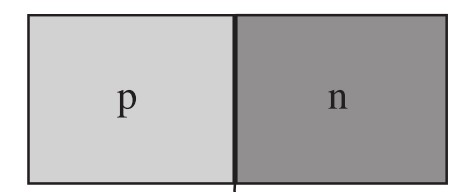
\includegraphics[width=0.3\linewidth]{pn-junction.jpg}
            \label{fig:pn-junction.jpg}
        \end{figure}
        \begin{figure}
            \centering
            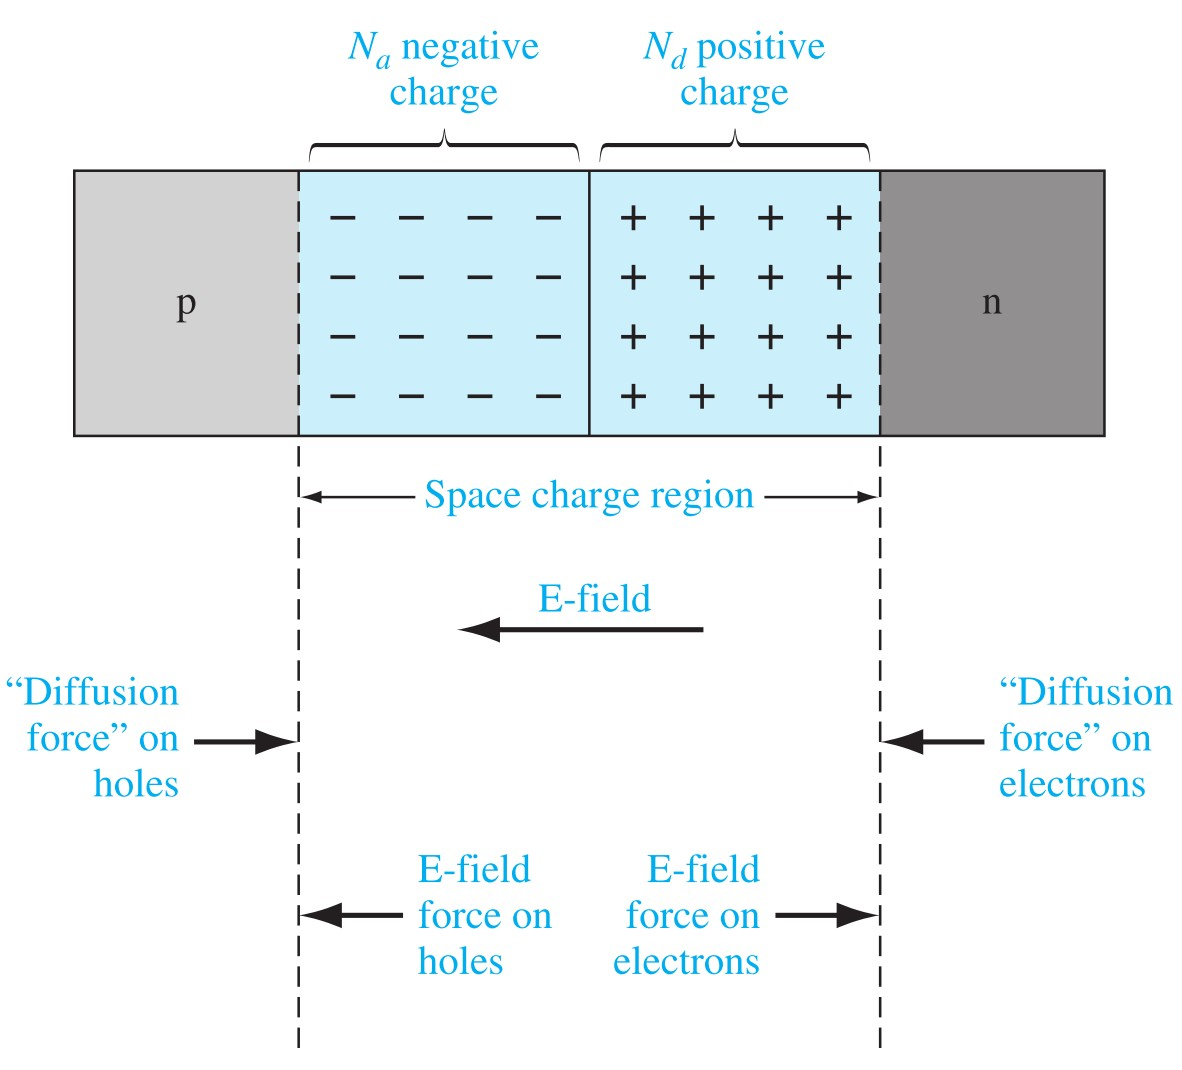
\includegraphics[width=0.6\linewidth]{Space-charge-region.jpg}
            \caption{\textit{space charge region} (\textit{depletion region})}
            \label{fig:Space-charge-region.jpg}
        \end{figure}
    \end{frame}

    \begin{frame} \frametitle{Energy-band Diagram}
        \begin{figure}[H]
            \centering
            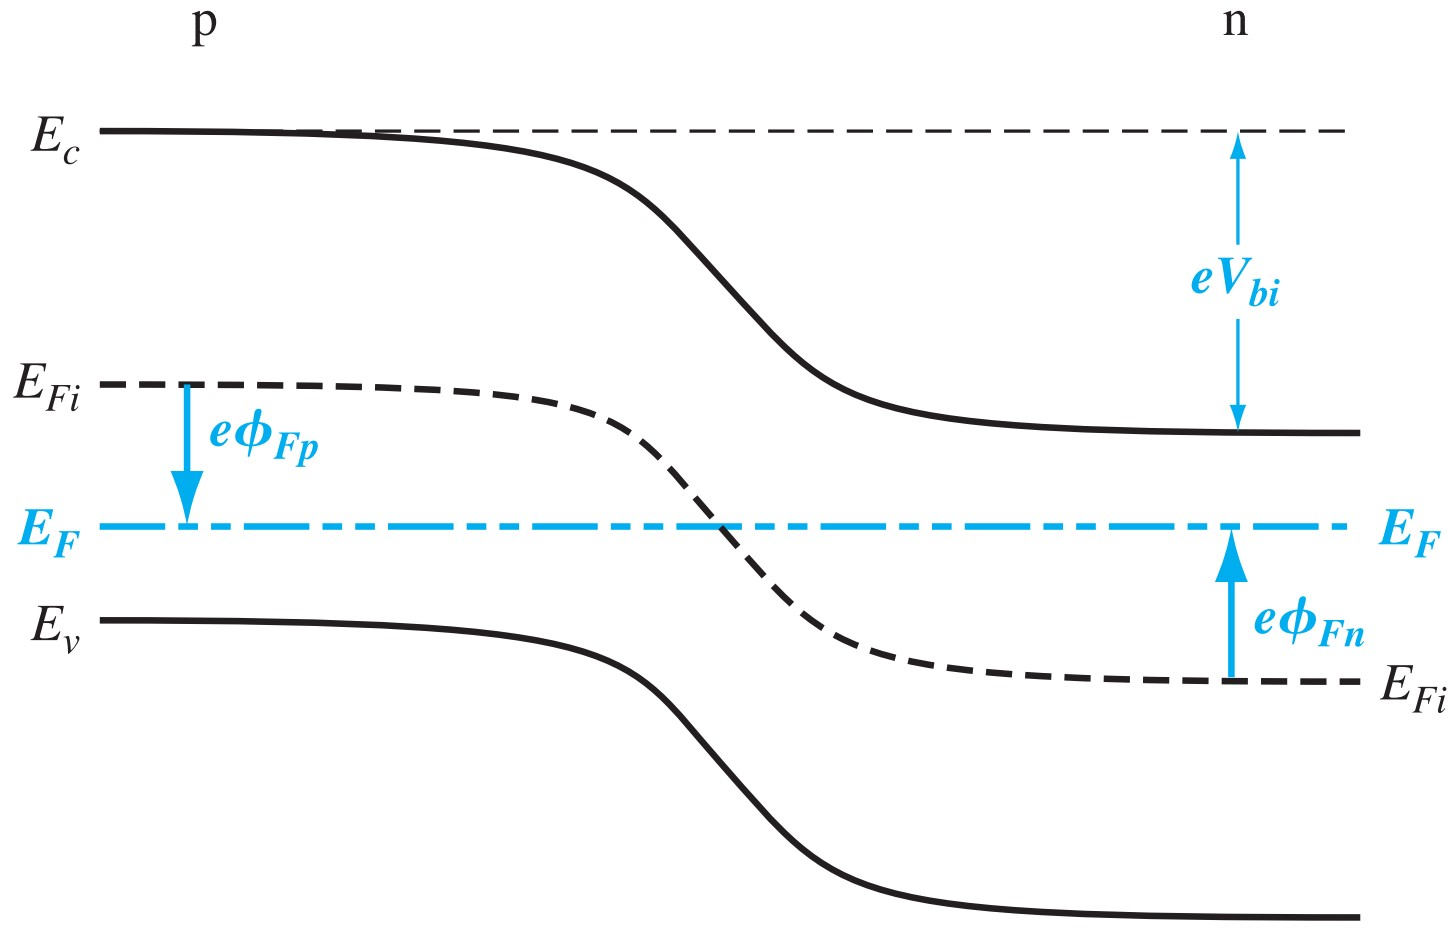
\includegraphics[width=0.6\linewidth]{pn-junction-energy-band-diagram.jpg}
            \caption{Energy-band diagram of a pn junction in thermal equilibrium}
            \label{fig:pn-junction-energy-band-diagram.jpg}
        \end{figure}
        $V_{bi}$: built-in potential barrier.
    \end{frame}

    \begin{frame}[t] \frametitle{Built-in Potential Barrier}
        \begin{figure}[H]
            \centering
            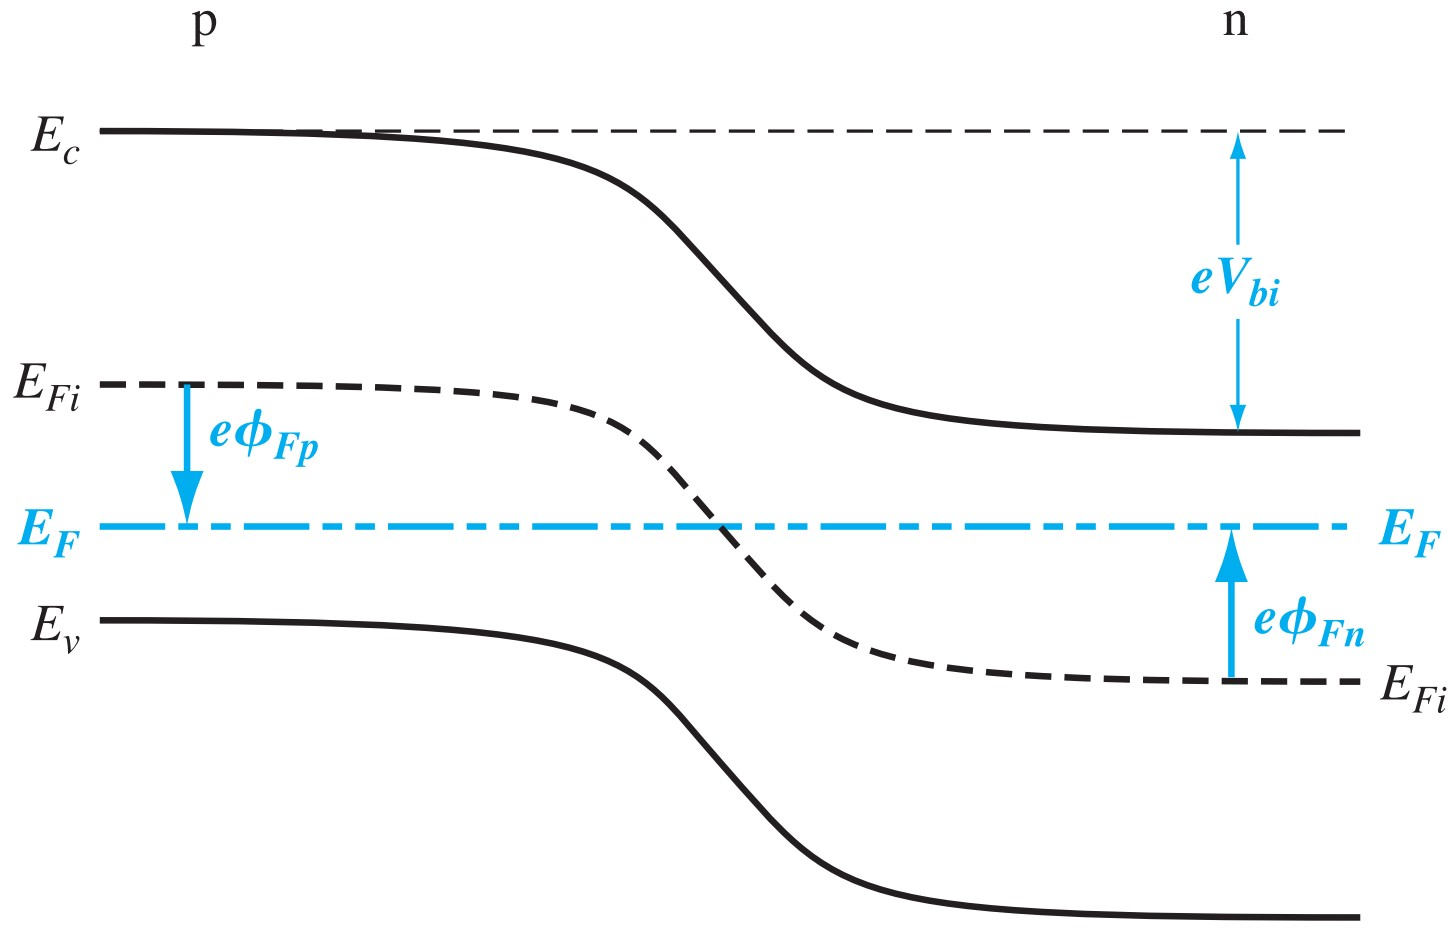
\includegraphics[width=0.5\linewidth]{pn-junction-energy-band-diagram.jpg}
            \label{fig:pn-junction-energy-band-diagram-2.jpg}
        \end{figure}
        \begin{equation*}
            \color{pink}
            \begin{aligned}
                V_{bi} &= |\phi_{Fn}| + |\phi_{Fp}| \\
                &= \frac{kT}{e} \ln \left( \frac{N_a N_d}{n_i^2}  \right) = V_t \ln\left( \frac{N_a N_d}{n_i^2}  \right) \quad (\text{not recommended})
            \end{aligned}
        \end{equation*}
        $V_t = kT / e$ defined as the thermal voltage.
    \end{frame}

    \begin{frame} \frametitle{Zero Applied Bias}
        \begin{minipage}{\linewidth}
            \begin{minipage}[b]{0.49\linewidth}
                \begin{figure}[H]
                    \centering
                    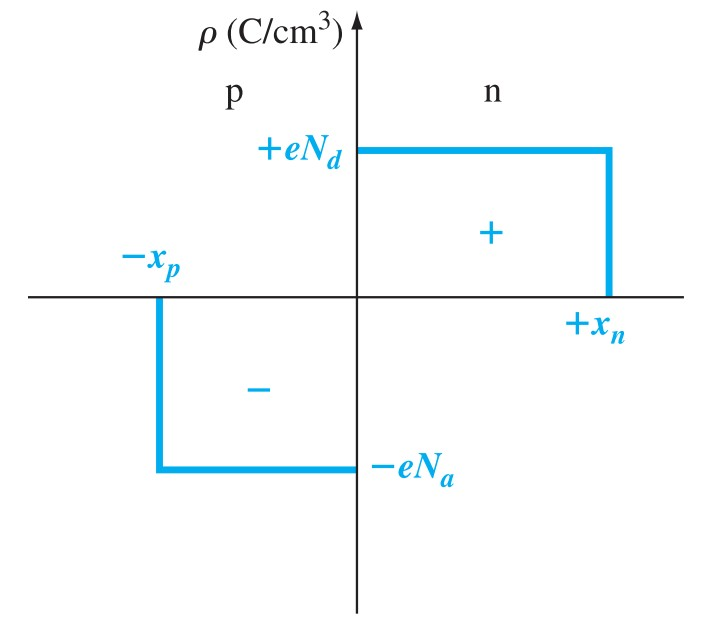
\includegraphics[width=0.95\linewidth]{Space-charge-density.jpg}
                    \caption{space charge density}
                    \label{fig:Space-charge-density.jpg}
                \end{figure}
                \begin{equation*}
                    N_a x_p = N_d x_n
                \end{equation*}
            \end{minipage}
            \begin{minipage}[b]{0.49\linewidth}
                \begin{figure}[H]
                    \centering
                    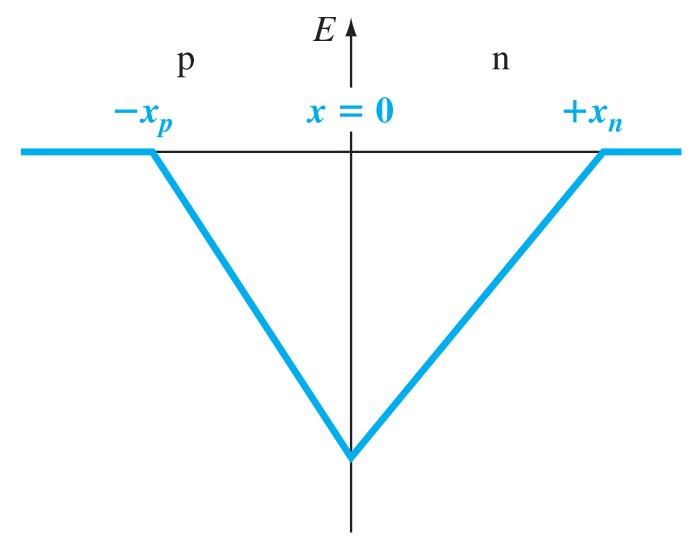
\includegraphics[width=0.95\linewidth]{pn-junction-electric-field.jpg}
                    \caption{electric field}
                    \label{fig:pn-junction-electric-field.jpg}
                \end{figure}
                \begin{equation*}
                    |k| = \frac{e N_{a/d}}{\varepsilon_s} 
                \end{equation*}
            \end{minipage}
        \end{minipage}
    \end{frame}

    \begin{frame} \frametitle{Zero Applied Bias}
        \fbox{
        \begin{minipage}{0.95\linewidth}
            \begin{equation*}
                N_a x_p = N_d x_n
            \end{equation*}
            \begin{equation*}
                \begin{aligned}
                    x_n &= \sqrt{\frac{2 \varepsilon_s \left( V_{bi} + V_R \right)}{e} \left[ \frac{N_a}{N_d}  \right]\left[ \frac{1}{N_a + N_d}  \right]} \\
                    x_p &= \sqrt{\frac{2 \varepsilon_s \left( V_{bi} + V_R \right)}{e} \left[ \frac{N_d}{N_a}  \right]\left[ \frac{1}{N_a + N_d}  \right]}
                \end{aligned}
            \end{equation*}
            \par $\varepsilon_s = \varepsilon_r \varepsilon_0$, where $\varepsilon_0 = 8.85 \times 10^{-14} F \cdot cm^{-1}$.
            \par $\varepsilon_r = 11.7$ for $Si$.

            \begin{equation*}
                W = x_n + x_p = \sqrt{\frac{2 \varepsilon_s \left( V_{bi} + V_R \right)}{e}  \left[ \frac{N_a + N_d}{N_a N_d}  \right]}
            \end{equation*}
        \end{minipage}
        }
    \end{frame}
    \begin{frame} \frametitle{Zero Applied Bias}
        \fbox{
        \begin{minipage}{0.95\linewidth}
            \begin{equation*}
                E = \left\{
                    \begin{aligned}
                        - \frac{eN_a}{\varepsilon_s} (x + x_p),\quad & - x_p \le x \le 0 \\
                        \frac{eN_d}{\varepsilon_s} (x_n - x),\quad & 0 \le x \le x_n  
                    \end{aligned}
                \right.
            \end{equation*}
            \begin{equation*}
                \begin{aligned}
                    |E_{max}| &= - \frac{eN_d x_n}{\varepsilon_s} = - \frac{e N_a x_p}{\varepsilon_s} \\ 
                    &= - \frac{2 (V_{bi} + V_R)}{W} 
                \end{aligned}
            \end{equation*}
            \begin{equation*}
                \phi(x) = - \int E(x) \d x
            \end{equation*}
        \end{minipage}
        }
    \end{frame}

    \begin{frame} 
        \begin{center}
            \Large\textcolor{blue}{End}
        \end{center}
    \end{frame}
\end{document} 